\section{Сравнение представления геометрии в GEANT/ROOT и САПР}\label{sec:ROOTvsCAD}

Разница между двумя способами описания геометрической информации в САПР и пакетах моделирования прохождения частиц через материал GEANT/ROOT заключается в двух пунктах. Во-первых, отличается способ задания геометрических форм. В САПР применяется граничное представление (BREP), для описания которого используются понятия типа <<поверхность>>, <<грань>>, <<ребро>>, <<кривая>>, и за которыми стоят соответствующие уравнения, описывающие эти объекты в пространстве. В GEANT/ROOT применяется конструктивная твердотельная геометрия (CSG), которая оперирует понятиями <<примитив>> и <<Булева операция>>. Очевидно, что и за этими объектами также стоят конкретные уравнения, описывающие кривые и поверхности, однако есть существенное различие описанное ниже. Во-вторых, отличается способ задания взаимоотношения форм в пространстве. В САПР, по аналогии с тем, как человек воспринимает окружающий мир, присутствует некоторое бесконечное окружающее пространство без материала, а все предметы находятся в этом пространстве. Невозможна такая ситуация, чтобы один объект находился внутри другого --- в таком случае подразумевается, что во втором есть соответствующая полость, освобождающая место под первый объект. При этом получается, что границы двух тел, стоящих рядом, совпадают, т.е происходит дублирование информации. \todo В силу математики это приводит к неприятным эффектам. \todo В GEANT/ROOT для описания взаимоотношения форм используется иерархия объёмов. Это объясняется тем, что такой метод более удобен для описания геометрии, где главной задачей является однозначное задание материала в каждой точке пространства. Вводится понятие объёма --- сущности, имеющей форму и материал. Из всех объёмов выбирается один, называемый объёмом верхнего уровня, а остальные помещены либо в него, либо в какой-то другой, формируя таким образом дерево объёмов. При этом не происходит дублирования границ и нет упомянутых выше эффектов.

\subsection{Представление геометрии в САПР}\label{sec:geoCAD}

%Ссылка на Голованова должна появиться где-то
В BREP есть два типа понятий --- геометрические (<<точка>>, <<кривая>>, <<поверхность>>) и топологические (<<вершина>>, <<ребро>>, <<грань>>). <<Точка>> --- это тройка координат в некоторой системе координат. <<Кривая>> --- это уравнение, задающее множество точек, принадлежащих данной кривой. Кривую удобно описать с помощью параметрического уравнения от одной переменной. <<Поверхность>> --- это уравнение, задающее множество точек, принадлежащих данной поверхности. Соответственно, поверхность удобно описать с помощью параметрического уравнения от двух переменных. Топологические сущности задаются на базе геометрических. <<Вершина>> лежит в некоторой геометрической точке. <<Ребро>> лежит на некоторой геометрической кривой и ограничено двумя вершинами. Очевидно, что эти вершины должны принадлежать кривой, то есть и соответствующие геометрические точки должны принадлежать кривой. <<Грань>> лежит на некоторой поверхности и ограничена замкнутым циклом из рёбер. Также очевидно, что эти рёбра должны принадлежать поверхности, как и кривые, на которых они лежат, как и вершины и точки, ограничивающие эти рёбра. Замкнутая оболочка из граней с указанием внешних сторон этих граней ограничивает некоторую область пространства, называемую <<телом>>.

В соответствии с BREP параллелипипед (которому эквивалентен примитив box в CSG) задаётся следующим образом.\\

\begin{figure}[H]
\centering
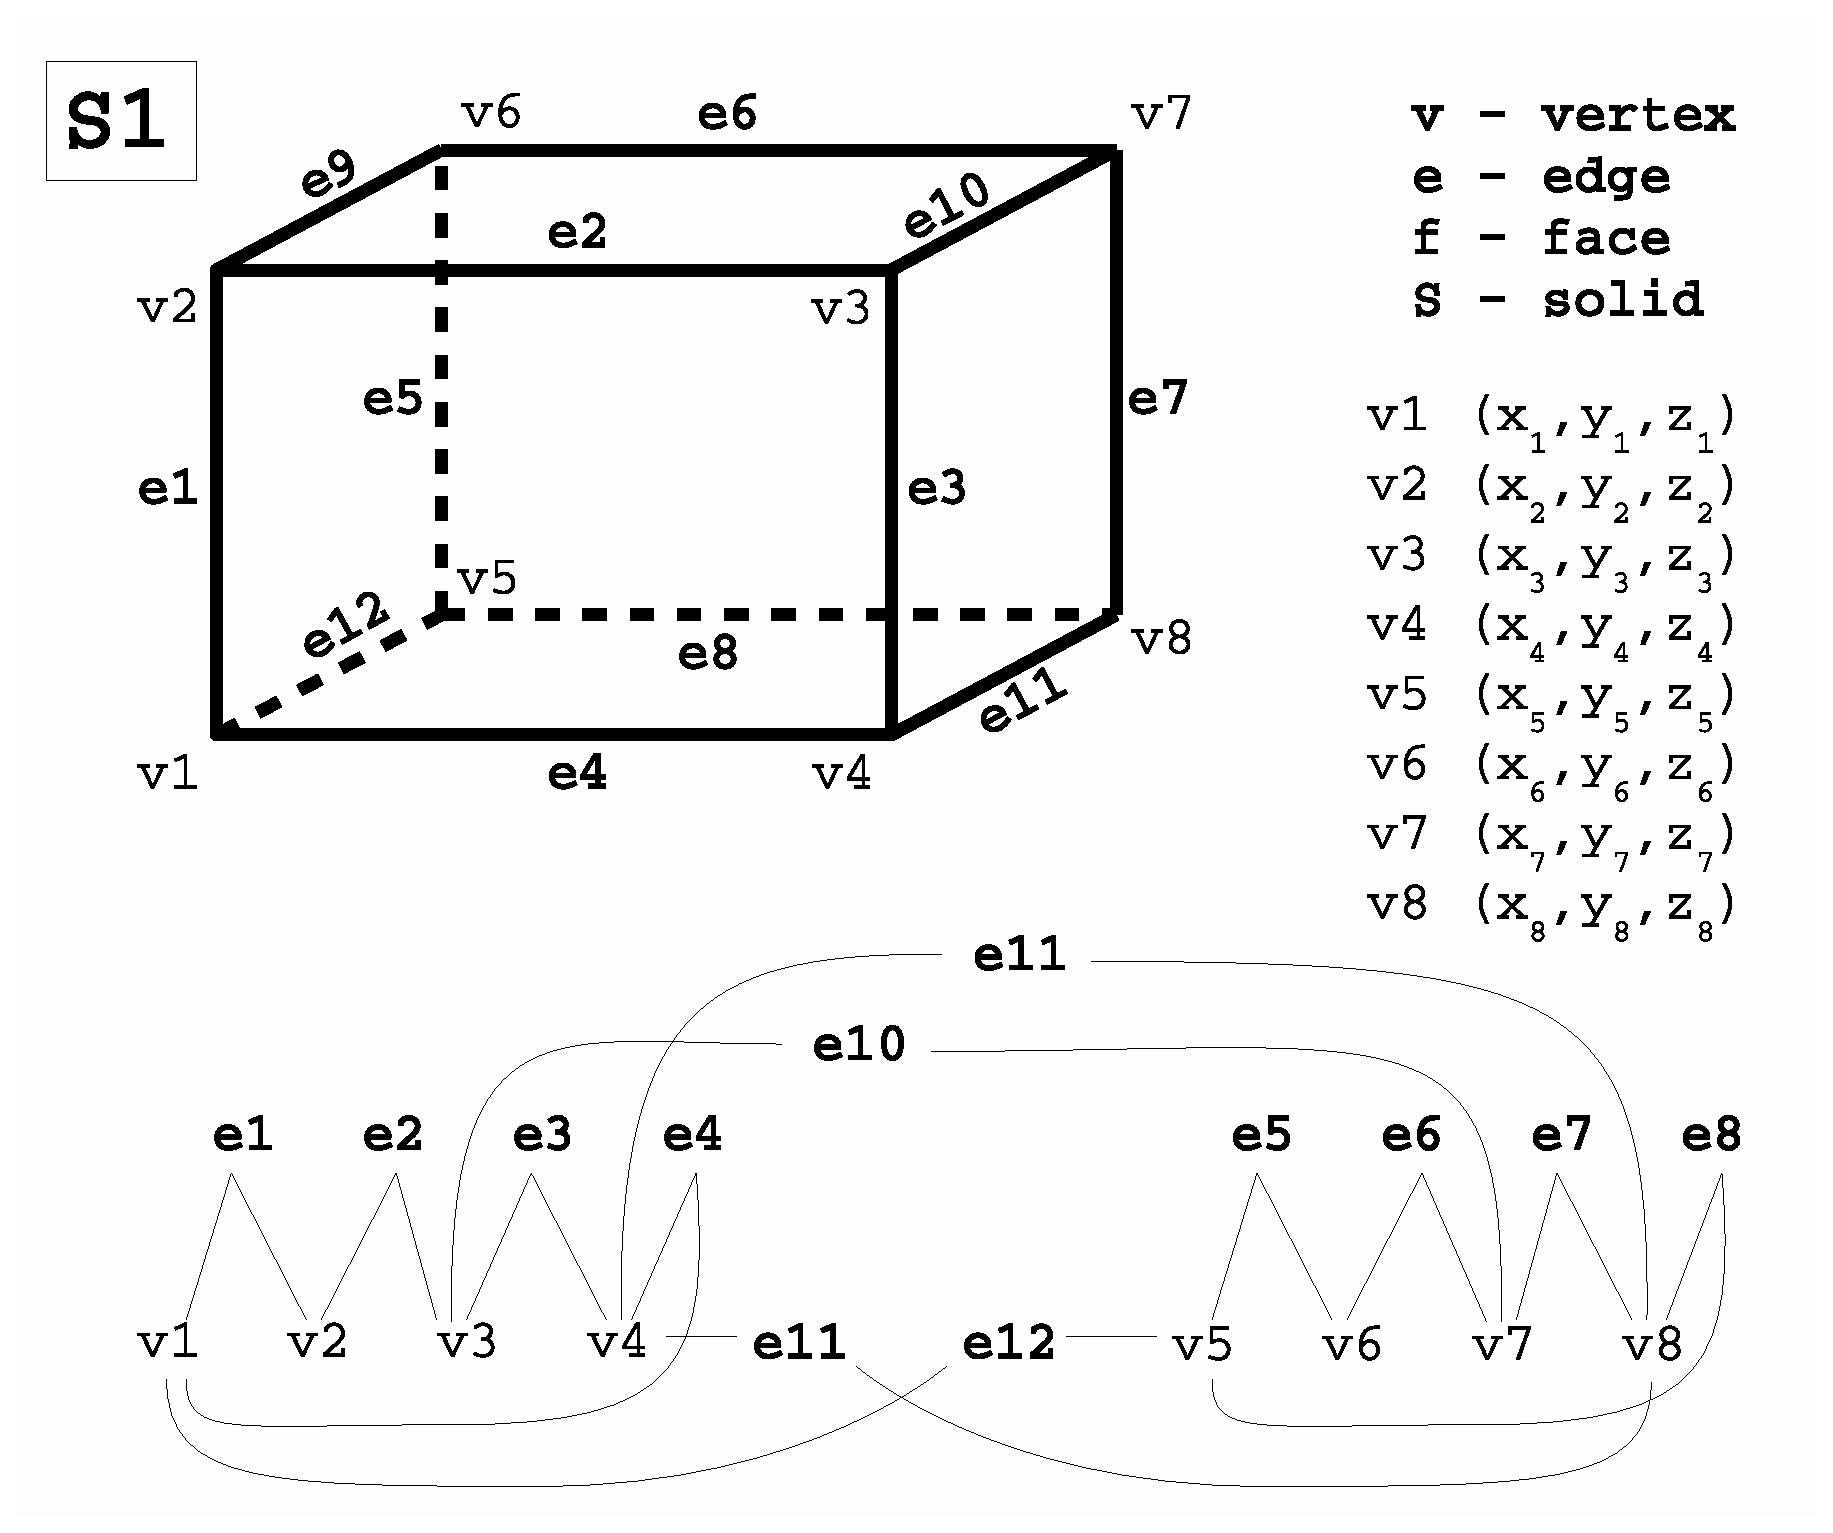
\includegraphics[width=0.7\textwidth]{pictures/BREPbox1.eps}
\caption{Описание вершин и рёбер примитива box методами BREP.}
\label{fig:BREPbox1}
\end{figure}

\begin{figure}[H]
\centering
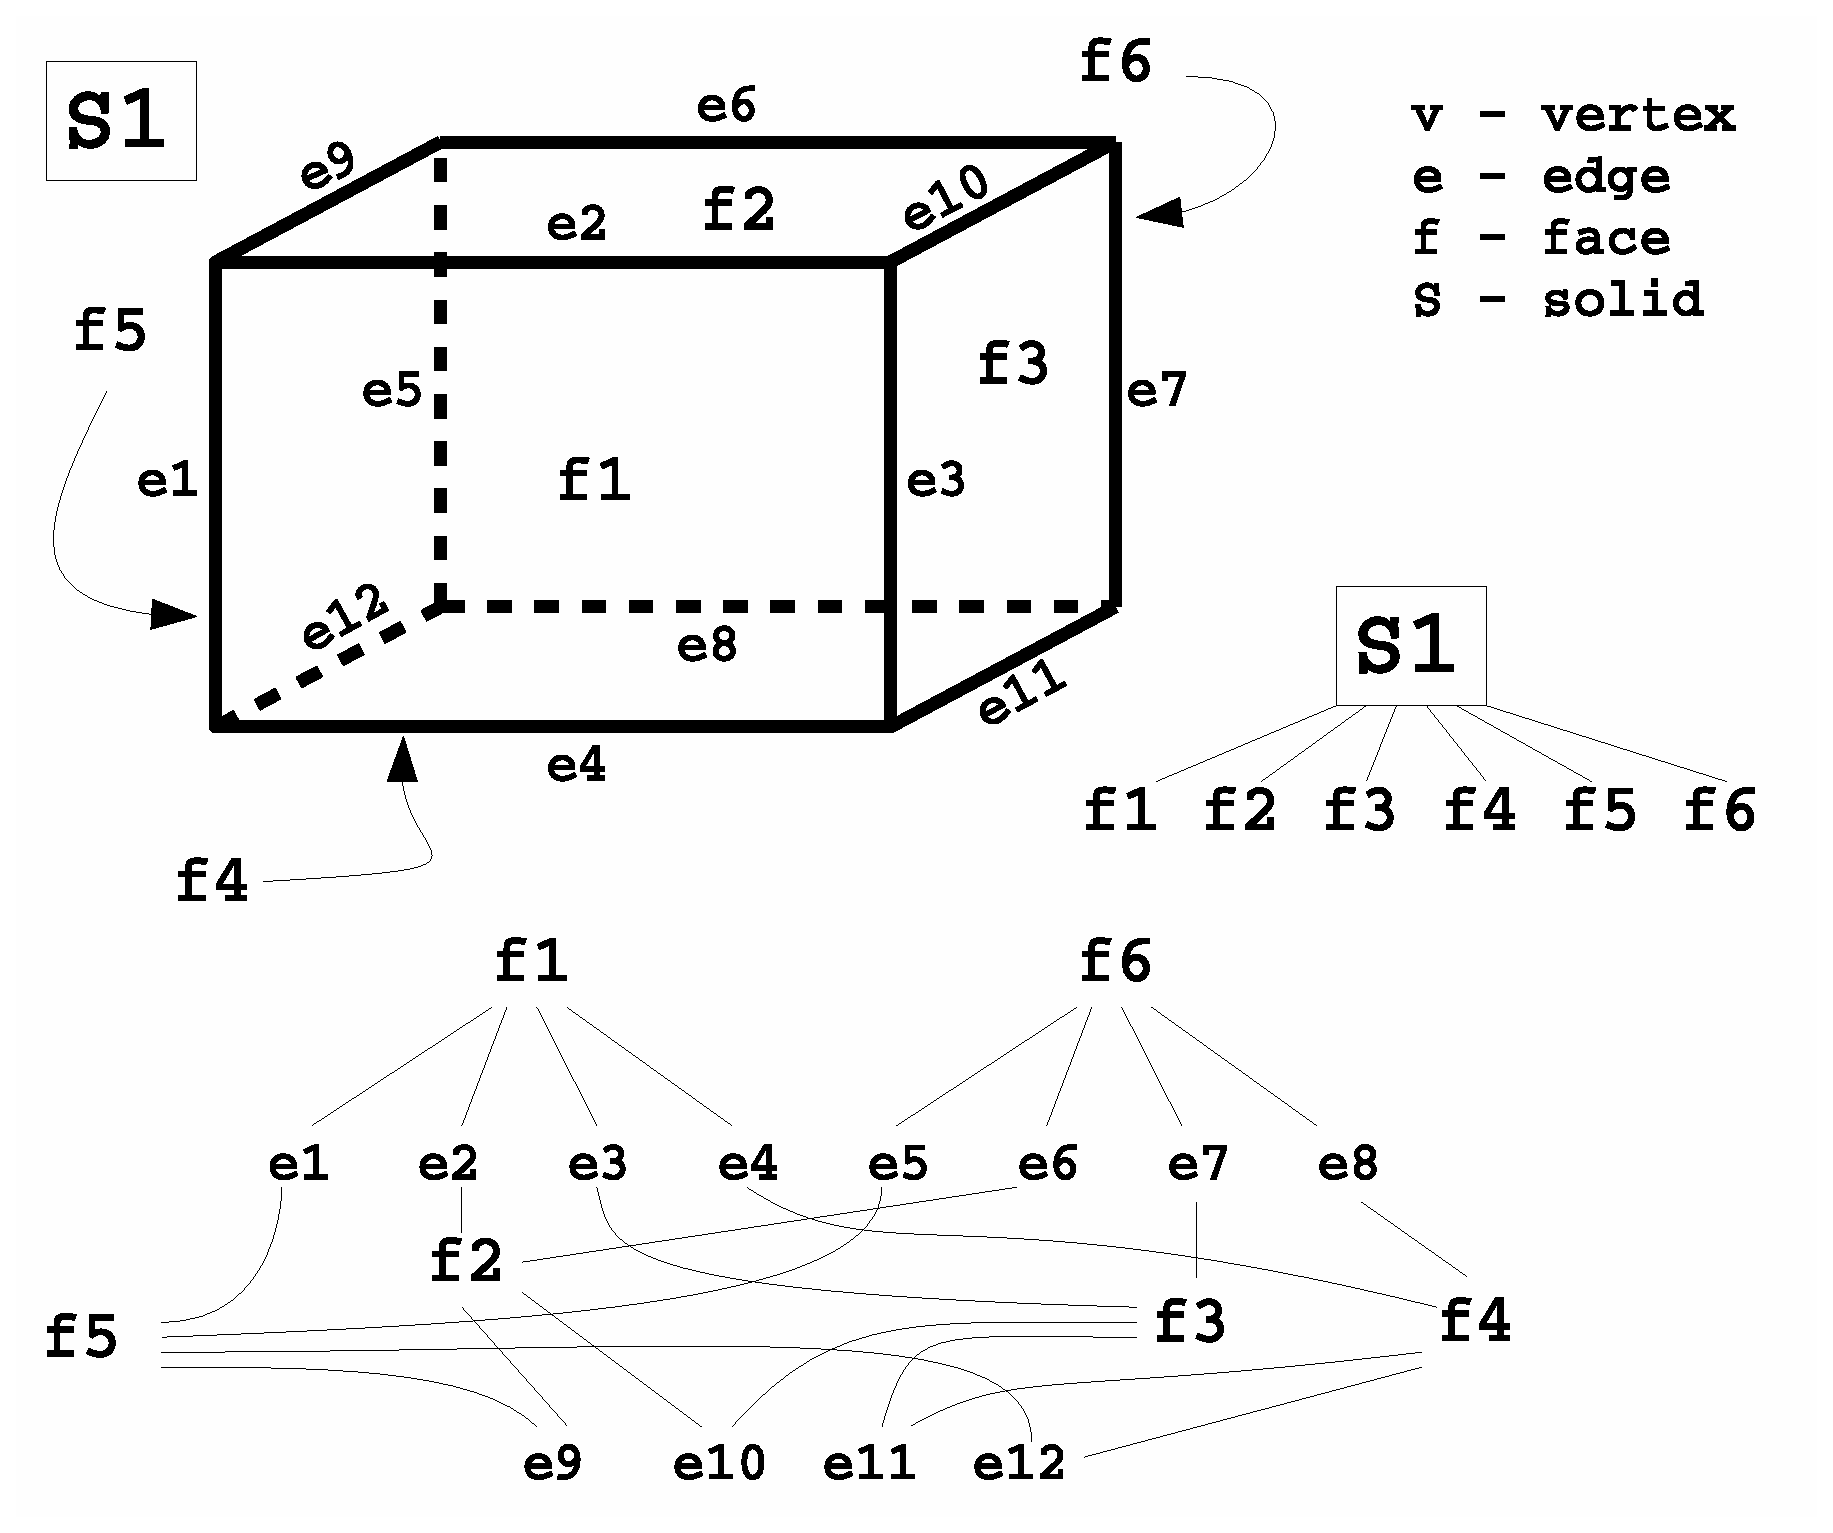
\includegraphics[width=0.7\textwidth]{pictures/BREPbox2.eps}
\caption{Описание граней и тела примитива box методами BREP.}
\label{fig:BREPbox2}
\end{figure}

\todo \textbf{Краткое описание картинки}

Стоит однако отметить, что человек, создающий геометрическую модель в САПР, хотя и может выполнять построения в соответствии с базовыми принципами BREP, чаще всего применяет интуитивно понятные формообразования, из которых система точно формирует BREP модель в памяти ЭВМ, которая также необходима для получения триангулированной геометрии для визуализации на дисплее ЭВМ. Есть 4 базовых формообразования и 4 им обратных (с вычитанием) --- <<выдавливание>>, <<вращение>>, <<протягивание>> и <<тело по сечениям>>. Многие другие формообразования, такие как фаски и скругления, разрезы, отверстия, внутри на самом деле являются лишь вариациями перечисленных. Последовательность формообразований, выполненных пользователем для получения итоговой формы, сохраняется в виде дерева построения модели, напоминающего историю построения, но позволяющего навигацию и редактирование. Дерево часто доступно пользователю в основном рабочем окне интерфейса САПР. Однако бывают случаи, когда история построения теряется, например при передаче модели из одной САПР в другую. Таким образом, в результате работы инженера получается модель, описанная с помощью BREP, и во многих случаях имеющая также и дерево построения.

В инженерной практике принято проектировать и соответственно строить 3d-модели, объединяя в сборки детали и другие сборки. Отсюда вытекает, что во многих САПР, в том числе в CATIA~v5, существуют стандартные объекты, обозначающие детали и сборки. Например в САПР CATIA~v5 существует отдельный тип документа CATPart для детали и отдельный тип документа CATProduct для сборки. Внутри документа типа CATPart есть минимальный набор обязательных элементов --- 3 стандартные взаимноперпендикулярные плоскости в начале системы координат детали и главное тело детали, по умолчанию называемое PartBody. В документе типа CATProduct присутствует возможность добавлять в качестве дочерних компонентов либо документы CATPart либо другие документы CATProduct. В~\ref{sec:Builder} описывается, как соотносятся перечисленные сущности CATIA~v5 с понятиями геометрической подсистемы GEANT/ROOT.

Во многих САПР, в том числе и CATIA~v5 присутствует возможность так называемого контекстного редактирования компонентов. Это означает, что пользователь во время работы над сборкой в документе типа CATProduct, имеющей в качестве дочерних компонентов детали в файлах типа CATPart, может также редактировать детали, не переключая активный документ. Эта возможность широко используется в ``CATIA-GDML geometry builder'' --- большая часть работы выполняется в контексте единственного продукта, что с точки зрения пользователя аналогично работе над всей экспериментальной установкой.

\subsection{Представление геометрии в GEANT/ROOT}\label{sec:geoROOT}

Для описания геометрических форм в пакетах GEANT/ROOT применяется CSG. В качестве строительных блоков в CSG используются примитивы из списка реализованных в системе. Список примитивов включает в себя как относительно простые примитивы типа параллелипипеда (box), сегмента цилиндра (tubs), сегмента конуса (cons), так и достаточно сложные, типа эллипсоида, параболоида, скрученных (twisted) примитивов. Принимая во внимание тот факт, что геометрия в GEANT/ROOT нужна для выполнения моделирования взаимодействия частиц с материалом, можно сказать, что примитив --- это объект, имеющий геометрическое представление и для которого реализовано решение геометрических задач, возникающих при моделировании. Среди таких геометрических задач можно отметить задачу нахождения расстояния до ближайшей границы примитива от некоторой точки внутри объёма, в одном заданном направлении или в любом возможном направлении. Эту задачу необходимо решать многократно в процессе проведения частицы для того, чтобы определить так называемый максимальный допустимый геометрический шаг. В результате моделирования физических процессов получается максимальный допустимый шаг из соображений физики. Для того чтобы собственно изменить координату частицы из этих двух шагов выбиратся минимальный. Каждый примитив, как в GEANT4, так и в ROOT, реализован как отдельный C++ класс, имеющий свои геометрические параметры среди членов данных, и решение описанных выше геометрических задач среди методов. Следует, отметить, что есть только параметры примитива, но нет никакого описания типа BREP. Уравнения границ фигурируют лишь в неявном виде в коде методов для решения геометрических задач. Более поробно примитивы описаны в~\ref{sec:Primitives}.

Форма может быть описана как результат Булевой операции над примитивами или другими Булевыми операциями. Есть три Булевы операции --- объединение (union), вычитание (subtraction) и пересечение (intersection). Булевы операции позволяют задать практически любую геометрическую форму, имеющую границы из тех, что применяются в примитивах. При этом не требуется дополнительной реализации решения геометрических задач, т.к. удаётся комбинировать то, что реализовано в примитивах. Более подробной применение Булевых операций для задания формы объёма описано в~\ref{sec:Boolean}.

Таким образом наблюдается некоторая аналогия между BREP и CSG, заключающаяся в том, что в любом случае сложное тело или базовый примитив имеет некоторые границы, заданные аналитическими выражениями. Корни этой аналогии лежат в фундаментальной математике. Однако решающая разница заключается в том, что для примитива эти границы чётко определены и имеется лишь ограниченное число параметров, позволяющих изменять форму примитива.

Вторая составляющая геометрического представления в GEANT/ROOT это иерархия объёмов. Введём понятия логического и физического объёмов, формы и материала. Логический объём, или просто объём это базовый элемент для построения иерархии объёмов. Объём описывает непозиционированный объект и всё, что находится внутри него. Объём характеризуется формой и материалом. Форма --- это заданные с помощью CSG границы пространства, по методу, описанному выше. Материал включает в себя описание химического состава, плотности, и т.д. При помещениb одного логического объёма в другой, например объёма $A$ в объём $B$, образуется так называемый физический объём, или узел, $B_1$, который обозначается взаимоотношение $A$ и $B$ как материнский-дочерний и характеризуется неоторой матрицей позиционирования $B$ внутри $A$.

\textbf{Продолжать!}\todo 